\apendice{Documentación técnica de programación}
\chaptermark{Documentación téc. de programación}
\label{ch:man-dev}

\section{Introducción} \label{sec:man-dev-intro}
Para que cualquier persona interesada en conocer, modificar o extender
el sistema desarrollado, este apéndice muestra los aspectos a tener en cuenta
para lograrlo.

Como los componentes del sistema, el sistema empotrado y la aplicación web,
tienen características tan diferentes cada uno necesita herramientas específicas
para su desarrollo.

Se detallan las particularidades de cada herramienta, los ajustes de
configuración, la estructura que toman los directorios con los ficheros
y los pasos necesarios para poner en funcionamiento el proyecto.



\section{Estructura de directorios} \label{sec:man-dev-struct}
Para empezar a trabajar con el proyecto lo primero que se necesita es una
copia del código fuente. La manera más sencilla de consultar y obtener el código
es acudir a los repositorios de GitHub. Hay un repositorio dedicado al \sw{}
del sistema empotrado \cite{webpage:repo-se} y otro para el \sw{} de la
aplicación web \cite{webpage:repo-aw}.


\subsection{Estructura de directorios del sistema empotrado}
\label{sec:man-dev-struct-se}
El código fuente del \sw{} del sistema empotrado toma la siguiente estructura:

\begin{description}
  \item[/] Directorio raíz, contiene el resto de directorios. Incluye el
  fichero LICENSE que contiene los términos y condiciones del licenciamiento
  del \sw{}. Además contiene un fichero de tipo MEX generado por el entorno
  de desarrollo (IDE) que sirve para configurar el \hw{} de la placa de
  desarrollo. Y el fichero Doxyfile que configura la herramienta de documentación.
  \item[/CMSIS/] Fuentes pertenecientes al Cortex Microcontroller Software
  Interface Standard (CMSIS). Proporciona interfaces al procesador y sus
  periféricos.
  \item[/amazon-freertos/] Fuentes pertenecientes a FreeRTOS, el RTOS usado por
  el sistema empotrado.
  \item[/board/] Fuentes autogenerados por el IDE y sus Config Tools que 
  permiten habilitar y configurar el \hw{} de la placa de desarrollo.
  \item[/doc/] Contiene la documentación del código y del proyecto.
  \item[/doc/amazon-freertos/] Documentación incluida con FreeRTOS.
  \item[/doc/lwip/] Documentación incluida con lwIP.
  \item[/doc/memoria/] Documentación del proyecto, la memoria descriptiva y
  sus apéndices.
  \item[/doc/html] Documentación del código fuente generada por Doxygen.
  \item[/drivers/] Fuentes con los controladores necesarios para trabajar con el
  \hw{}.
  \item[/lwip/] Fuentes relativos a lwIP, la implementación de la pila de 
  protocolos TCP/IP.
  \item[/source/] Código fuente del proyecto. A destacar, el fichero ``main.c''
  encargado del funcionamiento general del sistema. Están presentes los ficheros
  encargados de tratar con \hw{}. También se encuentran los ficheros de
  configuración.
  \item[/startup/] Código de arranque generado por el IDE.
  \item[/utilities/] Código generado por el IDE con utilidades auxiliares usadas
  para depuración o registro de eventos.
\end{description}


\subsection{Estructura de directorios de la aplicación web}
\label{sec:man-dev-struct-aw}
El código fuente del \sw{} de la aplicación web toma la siguiente estructura:

\begin{description}
  \item[/] Directorio raíz, contiene el resto de directorios. Incluye el
  fichero LICENSE que contiene los términos y condiciones del licenciamiento
  del \sw{}. Aquí se ubica el
  fichero ``pom.xml'' usando por la herramienta Maven para la gestión y
  construcción del proyecto.
  \item[/doc/] Documentación del código fuente generada por Javadoc.
  \item[/src/main/] Contiene todo el código perteneciente a la aplicación web.
  \item[/src/main/java/] Código Java de la aplicación web.
  \item[/src/main/java/es.ubu.alu.controller] \extranjerismo{Beans} del
  controlador.
  \item[[src/main/java/es.ubu.alu.controller.network] \extranjerismo{Beans} del
  controlador específicos para la red.
  \item[/src/main/java/es.ubu.alu.model] \extranjerismo{Beans} del modelo.
  \item[/src/main/webapp/] Contiene el fichero XHTML con el código de la
  interfaz web.
  \item[/src/main/webapp/WEB-INF] Contiene los ficheros XML usados por
  el servidor de aplicaciones.
  \item[/src/main/webapp/resources/] Recursos adicionales de la interfaz web.
  \item[/src/main/webapp/resources/css/] Contiene el fichero CSS que modifica el
  aspecto de la interfaz.
  \item[/src/main/webapp/resources/images/] Contiene las imágenes y otros
  recursos gráficos a usar por la interfaz.
\end{description}



\section{Manual del programador}
Para desarrollar el proyecto se han utilizado dos IDE diferentes, uno para cada
\sw{}. Aunque no es indispensable usar las mismas herramientas, a continuación
se muestra como obtener, instalar, configurar y utilizar las mismas herramientas
utilizadas durante el proyecto.


\subsection{MCUXpresso IDE} \label{sec:man-dev-mcuxpresso}

\subsubsection{Instalación de MCUXpresso IDE} \label{sec:instalacion-mcu}
El IDE se puede obtener gratuitamente desde la zona de Recursos para
desarrolladores de NXP \cite{webpage:mcuxpresso-ide}. El único requisito
establecido por NXP es tener una cuenta registrada, gratuita también, en su
sitio web.

Una vez iniciada la sesión y accedido al área de descarga se puede obtener
la versión más reciente del IDE. De ser necesario, también es posible descargar
una versión antigua desde la pestaña \extranjerismo{Previous}.

Tras aceptar los términos y condiciones de uso se muestran los enlaces de
descarga de los instaladores del IDE. 

\imagen{mcu_descarga}{Descarga de MCUXpresso IDE}

El instalador sigue el proceso de instalación habitual a la mayoría de programas.
Aceptar licencia de uso, indicar la ubicación del programa e informar
que se van a instalar controladores de depuración son los pasos más relevantes.

Concluida la instalación MCUXpresso solicita la ubicación del espacio de trabajo
o \extranjerismo{workspace} donde situar los proyectos. Cuando MCUXpresso
está listo para su uso presenta el aspecto habitual a cualquier otro IDE basado
en Eclipse IDE.

\imagen{mcuxpresso-wsp}{MCUXpresso recién instalado}

\subsubsection{Instalación de MCUXpresso SDK} \label{sec:instalacion-mcu}
MCUXpresso IDE lleva integrado las MCUXpresso Config Tools, sin embargo, es
necesario instalar MCUXpresso SDK, el kit de desarrollo de software (SDK),
que incluye los \extranjerismo{drivers}, \extranjerismo{middleware} y otras
utilidades necesarias para el desarrollo.

Las características del SDK están descritas en la web de NXP
\cite{webpage:mcuxpresso-sdk} al igual que las de MCUXpresso IDE. En cambio,
la descarga se realiza desde un sitio dedicado a la configuración de los SDK.

\imagen{sdk-download}{Sitio de MCUXpresso SDK Builder
\cite{webpage:mcuxpresso-sdk-builder}}

El sitio de configuración de SDK permite personalizar, o construir, un SDK
específico para la placa de desarrollo utilizada. Además permite seleccionar
que componentes incluir o no en el SDK.

Para poder descargar el SDK, NXP requiere iniciar sesión con una cuenta de
usuario de la misma manera que en la descarga del MCUXpresso IDE.

Dentro del configurador, el primer paso necesario consiste en buscar el
\hw{} para el que está destinado el SDK. En este caso, el \hw{} de desarrollo
va a ser la placa de desarrollo FRDM-K64F.

\imagen{sdk-selector}{Selección de la placa de desarrollo
\cite{webpage:mcuxpresso-sdk-builder}}

Seleccionada la placa de desarrollo falta configurar el SDK a las necesidades
del proyecto. La elección del sistema operativo puede variar entre
desarrolladores por lo que queda en su mano la elección. Por otro lado, el IDE
va a ser necesariamente MCUXpresso IDE.

Por último, hay que configurar el \extranjerismo{middleware} incluido con el SDK.
Los componentes mínimos a seleccionar son FreeRTOS y lwIP aunque no supone
ningún inconveniente elegir más componentes.

\imagen{full-sdk}{Resumen del SDK completo
\cite{webpage:mcuxpresso-sdk-builder}}

MCUXpresso IDE ofrece una vista con los SDK instalados. Para agregar el SDK
recién descargado basta con hacer clic derecho en dicha vista e importar el
fichero comprimido con el SDK. Como alternativa, también sirve arrastrar el
fichero a la vista para para importar el SDK.

\imagen{sdk-import}{Importación del SDK}

\imagen{sdk-imported}{Detalles del SDK correctamente importado}

\subsubsection{Importación del proyecto} \label{sec:importacion-proj}
Para empezar a trabajar con el proyecto falta importar una copia el código
fuente. Una opción consiste en importar el proyecto directamente desde una
carpeta con los ficheros o desde un fichero con el proyecto comprimido.

Copiarlo desde un repositorio es otra opción que permite obtener la versión
del código más reciente. El código del \sw{} del sistema empotrado se halla en
GitHub \cite{webpage:repo-se}.

\begin{figure}[!h]
  \centering
  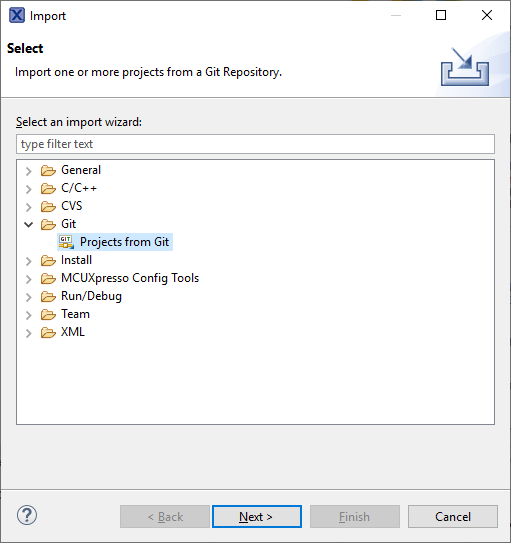
\includegraphics[height=0.45\textheight]{import}
  \caption{Importación del proyecto desde GitHub} \label{fig:import}
\end{figure}

La introducción de credenciales es necesaria para poder realizar
\extranjerismo{commit}, \extranjerismo{push} y el resto de operaciones de Git
con destino a GitHub, siempre y cuando se tengan permisos para operar en el
repositorio. Sino, solo se puede trabajar en local.

\begin{figure}[!h]
  \centering
  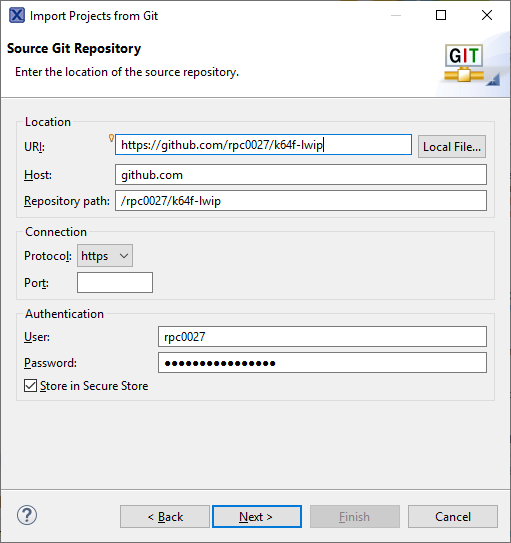
\includegraphics[height=0.45\textheight]{clone-git}
  \caption{Datos del repositorio} \label{fig:clone-git}
\end{figure}

Al aceptar la conexión con el repositorio, una serie de ventanas solicita más
información respecto a la ubicación del repositorio local, el proyecto a 
importar y si se usa el proyecto directamente o se genera uno nuevo.

Completado el proceso de importación el proyecto se encuentra listo 
trabajar con él.

\begin{figure}[!h]
  \centering
  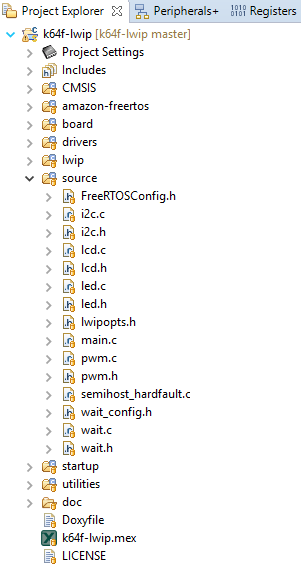
\includegraphics[height=0.45\textheight]{project-ready}
  \caption{Proyecto correctamente importado} \label{fig:project-ready}
\end{figure}

\subsubsection{Vista general de las Config Tools} \label{sec:config-tools}
Uno de los elementos diferenciadores de MCUXpresso respecto a IDE anteriores
es la incorporación de las Config Tools o herramientas de configuración.

En concreto, son tres herramientas que permiten configurar tres componentes
del sistema: pines, relojes y periféricos. Además, generan automáticamente el
código oportuno para habilitar e inicializar los dispositivos configurados. El
acceso a estas herramientas se consigue cambiando a sus respectivas perspectivas.

Con Pin Tools se configuran los pines del microcontrolador (MCU) enrutando
sus pines con la entrada o la salida adecuada. Los pines se pueden seleccionar y
enrutar en la vista ``Pins'' de la herramienta. Además, Pin Tools permite asociar
los pines en grupos. De esta manera es posible habilitar e inicializar grupos
de pines concretos simultáneamente.

\imagen{pin_selector}{Pines del grupo Ethernet en verde brillante}

Algunos pines requieren configuración adicional que se puede ajustar en la vista
``Routed Pins''.

\imagen{pin_config}{Configuración de los pines del grupo Ethernet}

La herramienta Clock Tools se utiliza para configurar los relojes del sistema
empotrado. En la vista ``Clocks Table'' se pueden introducir los valores de
configuración: frecuencias, multiplicadores, divisores... Por otra parte, la
vista ``Clocks Diagram'' muestra de forma gráfica la configuración establecida
en ese momento y también permite cambiar los ajustes sobre el diagrama
directamente.

\figuraApaisadaSinMarco{0.9}{clocks_diag}{Diagrama con los relojes del sistema}
{fig:relojes}{}

La última herramienta, Peripheral Tools, posibilita la configuración de los
dispositivos periféricos conectados al MCU. En función del periférico se
muestran las opciones específicas para cada uno de ellos.

\imagen{peripherals}{Configuración del periférico FTM}


\subsection{Eclipse IDE} \label{sec:man-dev-eclipse}
El desarrollo de la aplicación web requiere de varias herramientas aparte
del propio IDE. Una es el kit de desarrollo de Java, JDK, y la otra es el
servidor de aplicaciones GlassFish. Además, como se usa Maven para la gestión
del proyecto, también es necesaria su instalación.

\subsubsection{Instalación de JDK} \label{sec:jdk}
El JDK se puede obtener de la zona de descargas de Oracle \cite{webpage:javaee}.
Como el JDK es utilizado por el resto de herramientas, su descarga e instalación
se debe realizar en primer lugar. El instalador se encarga de todo el proceso a
excepción de la creación de una variable de entorno.

Para poder usar el JDK desde la consola de comandos, es necesario crear
una variable de entorno llamada ``JAVA\_HOME'' que apunte al directorio de
instalación del JDK. Después, hay que modificar el ``PATH'' al que hay
que añadir la nueva variable.

\subsubsection{Instalación de Maven} \label{sec:maven}
Maven está disponible en su sitio web \cite{webpage:maven}. La descarga consiste
en un fichero comprimido que no contiene ningún instalador. Para su uso, basta
con descomprimir el fichero en algún directorio del sistema. Después, para
localizar el directorio hay que crear una variable de entorno al igual que con
el JDK. En este caso, la variable se tiene que llamar ``M2\_HOME'' y también
tiene que ser agregada al ``PATH''.

\subsubsection{Instalación de GlassFish} \label{sec:glassfish}
La manera de instalar GlassFish es similar a la anterior. Hay que descargar un
fichero comprimido desde su sitio web \cite{webpage:glassfish}, descomprimir
el fichero en un directorio a elegir y que crear una variable que apunte a ese
directorio. En este caso, la variable de entorno toma el nombre de 
``GLASSFISH\_HOME'' y también se añade al ``PATH''.

\subsubsection{Instalación de Eclipse IDE} \label{sec:eclipse}
El instalador del IDE se puede obtener libremente desde el sitio de Eclipse
\cite{webpage:eclipse}. Como existen varias versiones de Eclipse, el instalador
permite escoger la versión requerida, en este caso, se selecciona ``Eclipse IDE
for Enterprise Java Developers''.

\imagen{installer}{Instalador de Eclipse IDE}

Después de terminar la instalación de Eclipse, es necesario instalar
una pequeña herramienta llamada Eclipse GlassFish Tools capaz de conectar
GlassFish con Eclipse. De esta manera es posible publicar las aplicaciones web y
controlar el estado del servidor directamente desde el IDE.

La herramienta se encuentra disponible tanto en el Eclipe Marketplace como
en el repositorio de la propia herramienta \cite{webpage:glassfish-tools}. Una
vez instalada, se puede configurar el servidor desde la vista ``Servers''.

\imagen{repository}{Instalación de las Eclipse GlassFish Tools}

\subsubsection{Importación del proyecto} \label{sec:importacion-proj-ee}
La importación del proyecto es similar a la descrita para MCUXpresso
\ref{sec:importacion-proj}, bien importando un fichero o bien descargándolo
desde GitHub \cite{webpage:repo-aw}.

\imagenancho{aw-imported}{Proyecto correctamente importado}{!h}{0.45}

\clearpage



\section{Compilación, instalación y ejecución del proyecto} \label{sec:exe}
\sectionmark{Compilación, instalación y ejecución}
Con los entornos de desarrollo y sus respectivos proyectos preparados es posible
compilar los códigos fuente. Dependiendo del \extranjerismo{software} a ejecutar
es necesario tomar diferentes caminos para su puesta en marcha.


\subsubsection{Compilación, escritura y ejecución del sistema empotrado}
\label{sec:exe-se}
Existen varias vías para compilar el código fuente. Una de ellas es hacer clic
derecho sobre el proyecto y en el menú contextual, pulsar sobre ``Build
Project''. Otra forma es pulsar sobre su icono correspondiente en la barra de
herramientas.

Para realizar la escritura, o \extranjerismo{flash}, de los binarios en el
sistema empotrado y que pueda ejecutarlos hay que lanzar desde el IDE la
operación de ``Debug''. Igual que la compilación, se puede hacer desde el menú
contextual o desde la barra de herramientas. Cabe decir que la operación de
depuración ejecuta automáticamente la de compilación, haciendo innecesario tener
que ordenarla manualmente.

La primera vez que se lanza un \extranjerismo{debug} el IDE solicita la
identificación de la placa de desarrollo. Para identificar la placa de
desarrollo hay que especificar el uso de ``SEGGER J-Link probes'', 
compatibles con OpenSDA, el adaptador serie y de depuración integrado en la
placa. 

\imagen{probes}{Reconocimiento de la placa de desarrollo}

\imagen{probed}{Placa de desarrollo reconocida}

Cuando la placa dispone del \sw{} arranca su ejecución. Al estar en modo de
depuración, la consola de depuración se activa y queda lista para mostrar los
mensajes enviados por la placa cuando corresponda.

\imagen{console}{Sistema en ejecución}


\subsubsection{Despliegue y ejecución de la aplicación web} \label{sec:exe-aw}
Como la aplicación web depende de un servidor de aplicaciones para funcionar,
se hace necesario desplegarla en uno antes de poder utilizarla.

Eclipse permite realizar el despliegue automáticamente. Además, permite
controlar el estado del servidor de aplicaciones pudiendo iniciarlo, detenerlo o
incluso, actualizar los ficheros de una aplicación ya desplegada.

En la vista ``Servers'' y haciendo clic derecho sobre el servidor GlassFish
se puede desplegar la aplicación pulsando en la opción ``Add and remove'' del
menú contextual. En la ventana que aparece después, se selecciona la aplicación
en el cuadro de la derecha y pulsando ``Add >'' queda configurada para ser
publicada en el servidor.

\imagenalto{add}{Aplicación configurada para ser publicada}{!h}{0.45}

Mientras el código de la aplicación no sea modificado, la aplicación tendrá el
estado de sincronizada. Si el código cambia, su estado indicará que necesita
publicada de nuevo.

\imagenancho{published}{Aplicación publicada}{!h}{0.9}

Si el despliegue se ha completado con éxito, ya es posible acceder a la
aplicación web desde un navegador cualquiera. La URL de la aplicación es:
http://localhost:8080/web-app/ .

\imagen{success}{Acceso a la aplicación web desde un navegador}

Con Maven se presenta otra forma de abordar la construcción y publicación de la
aplicación web. Ejecutando en el directorio raíz del proyecto el comando:
\begin{quotation}
  mvn package
\end{quotation}
Maven crea un archivo de tipo WAR, utilizados en Java para la distribución de
aplicaciones web, llamado ``web-app-1.0.war''. Ese archivo se puede publicar
en el servidor con el siguiente comando:
\begin{quotation}
  asadmin deploy web-app-1.0.war
\end{quotation}
En caso de que la aplicación ya estuviera desplegada, por ejemplo, porque se ha
desplegado desde Eclipse, el comando fallaría avisando de esta circunstancia.
De no haber errores, la aplicación web queda disponible para ser utilizada
usando la misma URL que en el caso anterior. 



%\section{Pruebas del sistema}